\begin{figure}[htbp]
\centering
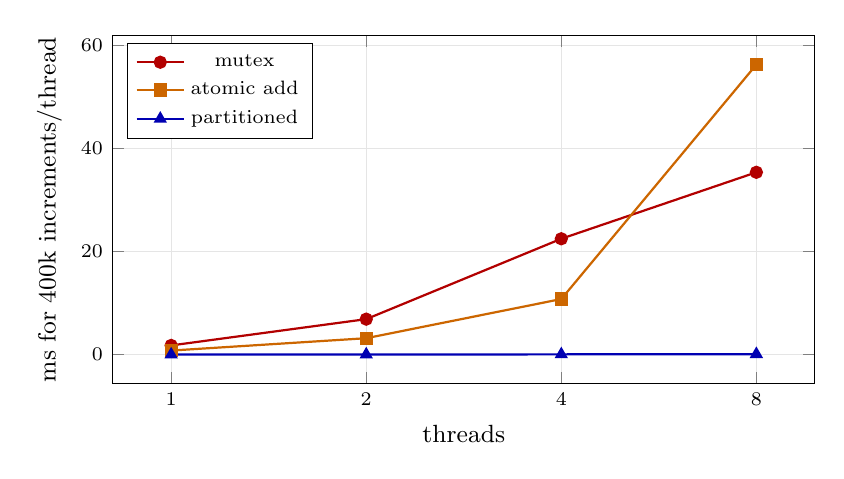
\begin{tikzpicture}
\begin{axis}[width=10.5cm,height=6cm,
  xlabel={threads}, ylabel={ms for 400k increments/thread},
  symbolic x coords={1,2,4,8}, xtick=data,
  grid=major, grid style={gray!20},
  tick label style={font=\scriptsize}, label style={font=\small},
  legend style={font=\scriptsize, at={(0.02,0.98)}, anchor=north west}]
\addplot[thick,mark=*,color=red!70!black] coordinates {(1,1.8)(2,6.9)(4,22.5)(8,35.4)};
\addplot[thick,mark=square*,color=orange!80!black] coordinates {(1,0.8)(2,3.2)(4,10.8)(8,56.3)};
\addplot[thick,mark=triangle*,color=blue!70!black] coordinates {(1,0.031)(2,0.032)(4,0.065)(8,0.109)};
\legend{mutex, atomic add, partitioned}
\end{axis}
\end{tikzpicture}
\caption{Real \texttt{ch13\_lockscale.c} on this laptop. Partitioning
is flat ($\sim$0.1\,ms) because nothing is shared. The honest
surprise: at 8 threads the atomic add is \emph{slower than the
mutex} --- the single contended cache line costs more than the lock.}
\label{fig:lockscale13}
\end{figure}
